\chapter{On Database Background}

\section{Databases}

A standalone database is not very useful as it is only some physical storage that never changes. To take the full advantage of it we need some means to define, create, maintain and control access to the database. That is purpose of a software called \definition{Database Management System (DBMS)}.

We already described why we want to use a database and roughly mentioned what are the pieces of data that we want to save there. 
Now let's take a look at what are differences between in database implementations and what to take in account when comparing database technologies.
That may be helpful when choosing the best suitable option for some specific data set to store or to see how storing of great amount of structured information can be approached. \\ 

The basic division of databases types is simple and binary - they are either Relational or Non-Relational.

There are Database Management Systems build around both, Relational Database Management System (RDBMS)

\subsubsection{Relational Databases}
A \definition{Relational Database} is a set of tables. A table consists of rows (also records) and columns. We can see such table as an object whose attributes are represented by columns and instances by rows. 
The important aspect is that relational tables tables carry both data that need to be stored by user and the relationships between the data as well. 
To store an atomic piece of data about instance a proper column is filled with a value.
Whereas to capture a relationship between objects the concept of keys is used. \\
A \definition{Key} is a subset of table's columns used for identifying a record. \\
A \definition{Primary Key} is a Key that non-ambiguously identifies a record in table and is used when referring to the record. \\
A \definition{Foreign Key} is a Key that uniquely identifies a record from a table (may be the same or a different one). \\
They are known also as SQL databases by the language - \definition{Structured Query Language (SQL)} which is used in RDBMS for managing data.

To be concrete, the most widely used relational database management systems are Oracle, MySQL, Microsoft SQL Server, PostgreSQL, IBM Db2 in this order. \footnote{The database technologies usage statistics are based on data from the most up to date version of website db-engines.com \cite{DatabaseEnginesStatistics19}.}

In this work will focus only on the databases that are of the relational kind, even though there are also NoSQL or Non-relational databases that do not follow the relational paradigm. 

The main reason behind this is the fact that NoSQL databases have a flexible schema or are schema-less (there is no point in determining a database schema when data types of attributes or keys) modeling of these databases quite a new discipline and is hard to find an intersection among different approaches to NoSQL modeling.
Also concepts of higher abstraction models are omitted. \cite{NoSQLDatabaseModeling}

The fact to consider is that once a database is Relational we more or less know what to expect from it. The structure of these databases has a fixed skeleton. So a tool that would extract metadata from relational data models is potentially more powerful as it can be applied to more database technologies than a similar tool aimed for some specific type of Non-Relational database. 

Lastly, despite the Non-Relational may be growing in numbers and became a serious alternative, as it suits some use-cases better, the Relational still are, and in the near future will be, far more widely used.

\subsubsection{Means of Database Access}

Databases can be managed directly using Database Management Systems by a user who is using query language for accessing a database. 
However third party, or application, programs need also access the DBMS. 
In our work two types of programs will be connecting to databases when fetching metadata - modeling tools when undergoing a reverse-engineering process and Manta Flow in the extraction phase.
A solution is to provide them with an application programming interface (API) that provides a set of methods available in the programming language that the application program was written in, so it can use them.
Most commonly when the API is called its implementation translates the request so that to a specific DBMS driver that it is passed after understands it and performs the desired action. \\

A \definition{Connection String} is a textual information used to identify a data source and establish a connection with it. It it is made of pairs of keywords and values separated by semicolon, the keywords are parameters of the connection.

\paragraph{APIs to DBMS}
\begin{itemize}
	\item Open Database Connectivity (ODBC)\\
		General, language independent, ER/Studio, PowerDesigner
	\item Java Database Connectivity (JDBC)\\
		The Java ecosystem, Manta Flow, PowerDesigner
	\item ADO.NET\\
		.NET Framework
\end{itemize}

\section{Database Modeling}
\label{chap:database_modeling}

Modeling is a crucial phase of database design process.
Developing a database is just like building a house. 
Every one will agree that no construction work can go without solid design and documentation. 
It would sound a bit strange to hire construction workers straight ahead and tell them that we need a house that has 5 rooms, some toilets and expect a good result. Most probably some building would be produced, but we will agree that expectations and requirements of the later inhabitant could not be met properly.
Surely there are good reasons why the usual steps are followed strictly.
Let us move on from the analogy to the database domain. \\
When deploying a database from a scratch we may think of two short term advantages. Firstly, the time needed to have data stored somewhere would be much shorter and secondly the initial cost of the system could be lower. \\
But over time both of the advantages will most likely, if the database is not ridiculously small, get outnumbered by problems that will begin to appear. Maintenance of a poorly designed system (or not designed at all) is expansive and leads to numerous outages.\\

There are good reasons to why modeling has its place in a database development process:

\begin{itemize}
	\item Higher quality.\\ Modeling push to thorough definition of the modeled problem. Once we know what to solve and what is the scope, it is much easier to come with different solutions and justify which of the proposed approaches is the most suitable one.
	
	\item Costs reduction.\\ Errors are identified thus can be caught in early stages, when they are easy to fix.
	
	\item Better documentation.\\ Data models form a nice piece of it, they are understandable by each of the involved stakeholders. When someone tries to understand the system, he can choose a data model on an appropriate level of abstraction that will introduce him the important aspects of the problem that suits his knowledge and qualification.
	
	\item Correctness.\\ Tracking whether high-level concepts were implemented and represented correctly in the end is made straightforward.
	
	\item Determining of consistency of the system.
	
	\item Deeper understanding.\\ During the design process we may learn a lot about properties of the data that we need or have and will be stored. These information are crucial for choosing an appropriate type of database, whether to stick with a relational database if so which DBMS is the one for us, or to look for a non-relational one.
\end{itemize}

\subsection{Data Model Perspectives}

\subsubsection{Vertical Division}

American National Standards Institute \cite{ANSIArchitecture75} came with a database structure called Three-schema architecture. It is formed by:
\begin{itemize}
	\item External Level \\ Database as a user sees it, view of the conceptual level. 
	\item Conceptual Level \\ Point of view of the enterprise that the database belongs to.
	\item Physical Level \\ The actual implementation.
\end{itemize}

The idea behind the structure was to create three different views that are independent of each other. 
For example change of the implementation that is tied with physical level would not affect any of the remaining levels if the structures remained the same. 
The important aspect is that this structure is used to describe finished product, it does not say anything about the design process that leads to the product and should not be mistaken with the differentiation of data models that will be introduced.\\

On the other hand, to standardize process of designing a database Peter Chen\cite{Chen76theentity-relationship} identified four levels of view of data, where each of the levels has its important place: \\
\begin{enumerate}
	\item Information concerning entities and relationships which exist in our minds.
	\item Information structure-organization of information in which entities and relationships are represented by data.
	\item Access-path-independent\footnote{An \definition{access path} is a description how records stored in a database are retrieved by database management system\cite{AccessPathDefiniton}. The important part is that the path is specific for a DBMS technology.} data structure-the data structures which are not involved with search schemes, indexing schemes, etc.
	\item Access-path-dependent data structure.
\end{enumerate}

The categorization of data models have undergone some modifications, for example the first level is today omitted, to the one that is recognized nowadays. The differentiation takes takes into account  what is the audience that will work with a data model, whether it is someone who knows all about databases or a business person without technical background. The levels of abstraction used today\cite{SilberschatzKorthSudarshan10} are the following: 
\begin{itemize}
	\item Conceptual Data Models (High-Level) \\
	Reproduces real world objects along with their relationships and should be close to how business end-users perceive them.
	
	\item Logical Data Models (Implementation, Representational) \\
	In the middle between the two other model types there are representational data models which on the one hand are comprehensible by end-users and on the other hand are not too abstract so that they can be used as documentation for an actual database implementation of the modeled data.
	
	\item Physical Level Data Models(Low-Level) \\
	In contrast to conceptual models the physical ones are tied with how data are stored physically at storage media showing all specific internal details that may be overwhelming in the case that the reader is a computer specialist.
\end{itemize}


\subsubsection{Horizontal Division}

\subsubsection{Relational Data Model}

A relational database is a direct implementation of a relational data model. A reader should be already familiar with the concepts used in the models from the sections describing terminology of SQL databases. All the terms such as table, column, entity, record and keys originate in the definition of relational data model \cite{Codd69}.

\subsubsection{Entity-Relationship Data Model}

The \definition{entity-relationship (ER) data model} was the direct answer for the four level architecture\cite{Chen76theentity-relationship} that covers the highest two levels and may be a basis for unified view of data. \\
It was an opposition to the three major data models that were used - relational, network and entity set model. His aim was to bring a data model that would reflect real-world objects and relations between them naturally, while having advantages of all the three already existing models. The mission seems to be successful as years have proven the ER data model to be the most suitable one for conceptual data modeling. Moreover, ER data models are used most commonly in logical data modeling as well.

\subsubsection{Enhanced-Entity-Relationship Data Model}

An extended version of ER data model was introduced later - \definition{enhanced-entity-relationship (EER) data model}. The main change is that concept sub-classes and super-classes, known as inheritance or is-a relationship, between entities was brought. \\ 

\TODO{conclusion}
Conceptual and logical data models are usually represented by ER data models. 
The question is what specific data model type is used for physical models. 
As the most low-level model type is tied directly with how a database is organized, physical models must obey the structure of database.

\subsection{Conceptual Data Model}

The purpose of a conceptual data model is to project to the model real-world and business concepts or objects. \\

\subsubsection{Characteristics}
\begin{itemize}
	\item Aimed to be readable and understandable by everyone.
	\item Is completely independent of technicalities like a software used to manage the data, DBMS, data types etc.
	\item Is not normalized.
\end{itemize}

A real world object is captured by an \definition{entity} in conceptual model. \\
For further description of objects that we are interested in \definition{attributes} are used, those are properties of entities. Only the important ones are listed. \footnote{Definitions varies and in some literature can be even found that a conceptual entity lacks attributes. We assume that the entity can contain important attributes as it is more common interpretation and modeling tools have attributes support on conceptual layer as well.} \\
Also \definition{relationships} between objects are necessary to provide full view of the section of the world that a data model resembles. \\

To illustrate it on an example, if our modeling domain is education, then an entity may be a teacher or lesson. 
A lsalary number would be an information to store when describing teacher, making it an attribute.
Having lectures captured in our data model, it is really fundamental to see what lesson is taught by who, that would be captured using relationships.

\begin{figure}[H]
	\centering
	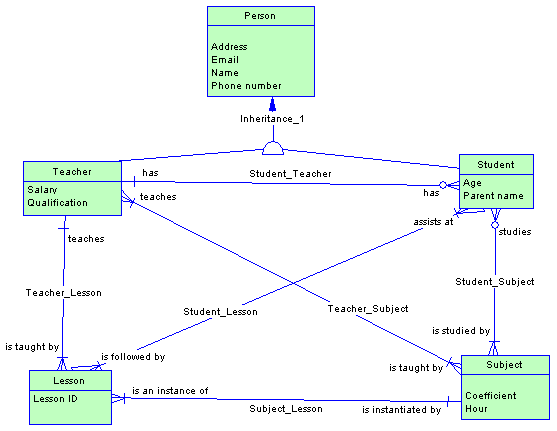
\includegraphics[width=10cm]{../img/Conceptual_Model_PowerDesigner}
	\caption{\TODO{Conceptual diagram}\cite{PowerDesignerDocumentation}}
\end{figure}

\subsection{Logical Data Model}

Keeping its structure generic a logical model extends the objects described in a conceptual data model making it not that easy to read but becomes a good base documentation for an implementation. Data requirements are described from business point of view.

\subsubsection{Characteristics}
\begin{itemize}
	\item Independent of a software used to manage the data or DBMS.
	\item Each entity has the primary key.
	\item Foreign keys are expressed.
	\item Data types description is introduced (but in a way that is not tied with any specific technology).
	\item Normalized up to \TODO{third normal form}.
\end{itemize}
\definition{Entities}, \definition{attributes} and \definition{relationships} from a conceptual model are present on this layer as well. Relationships are not that abstract as before and keys that actually make relationship happen between entities are added as their attributes.

\begin{figure}[H]
	\centering
	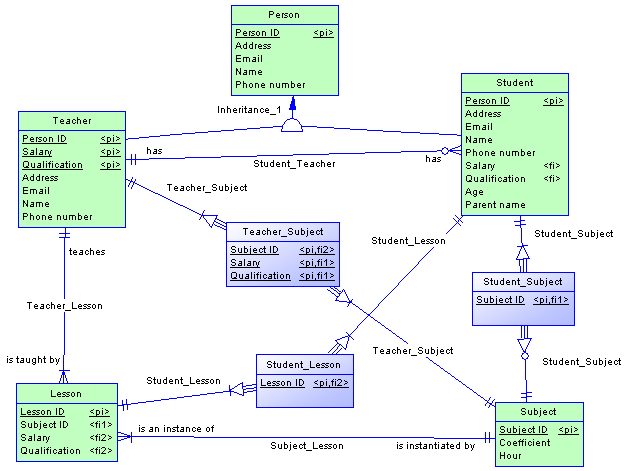
\includegraphics[width=10cm]{../img/Logical_Model_PowerDesigner}
	\caption{\TODO{Logical diagram}\cite{PowerDesignerDocumentation}}
\end{figure}

\subsection{Physical Data Model}

A physical data is a description of a database implementation so it is necessarily tied with one specific database technology as it should have one-to-one mapping to actual implementation. Its main message is to communicate how the data are stored.

\subsubsection{Characteristics}
\begin{itemize}
	\item Exact data types (DBMS specific) and default values of columns are outlined.
	\item DBMS's naming conventions are applied on objects.
	\item Constraints are defined (eg. not null, keys, or unique for columns).
	\item Contains validation rules, database triggers, indexes, stored procedures, domains, and access constraints.
	\item Normalization in order to avoid data redundancy or de-normalized if performance increase is reflected in the model.
\end{itemize}

Objects in physical models should reflect database organization and at the same moment related higher-level concepts should be transformable to physical level. \definition{Tables} should store records that corresponds to logical entities and \definition{columns} represent previously described attributes in memory.
Commonly schemas\footnote{Plural of the word schema is schemata but in literature about database design the word schemas is used} are present. A \definition{schema} is basically container for tables that logically groups them. Users have usually schemas assigned and can access only the tables contained in those schemas.

\begin{figure}[H]
	\centering
	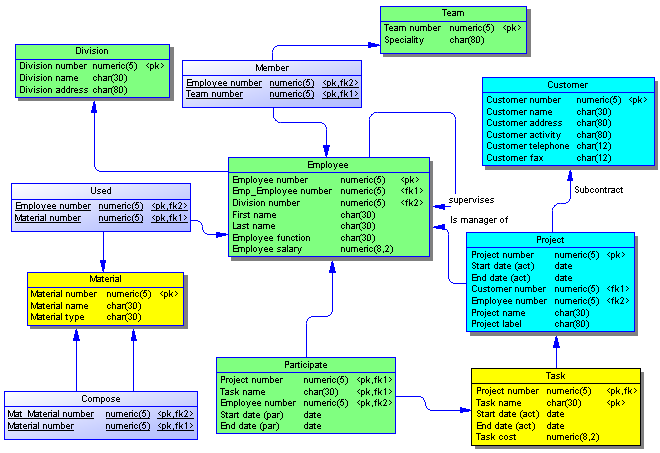
\includegraphics[width=10cm]{../img/Physical_Model_PowerDesigner}
	\caption{\TODO{Physical diagram}\cite{PowerDesignerDocumentation}}
\end{figure}

\subsection{Relations Between the Models}

We described what the role of each of the layers in a database design process is.
Now we will show that the data models are somehow connected vertically and what are the implications.

When talking about vertical divisions, we should think about how database design can proceed.

The basic approach is the \definition{top-down approach} to database modeling.
It is natural to start with a general idea what should a database store and what are the relations between stored object. 
End-user defines this high-level logic and as time goes importance of a database designer grows until he is at full charge and develops a complete database. It is the most common case of database development when a client identifies a high-level need for a database and hires an expert in this domain to make it happen.

The other way to create full view of a database is the \definition{bottom-up approach}. It can be harder to imagine what would be use-cases for this approach, but there are some problems that are bottom-up in nature. A nice real world example of bottom-up strategy is how doctors work. 
They start with "low-level" details such as symptoms and they're trying to build the whole image of patient's condition. So in the field of software data elements are firstly identified and after they are logically grouped to form bigger units, entities, and so on until the full hierarchy is known.

\subsubsection{Maps-to Relation}

In order to capture how high-level concepts are actually realized by more precise object a relation that we will call \definition{maps-to} is used. The relation leads between objects that are semantically equivalent on different levels of abstraction, sometimes even mapping between objects on the same layer are allowed but we will not consider this, as we consider it be mixing two different concepts together - data modeling with data lineage. To be more precise what we mean by semantically equivalent objects in data models is that we will assume maps-to edges solely source is model and target is model, entity and table, attribute and column, or the other way around.
Following these mapping links is extremely useful when a person wants to gain an overall overview of the system and comprehend it. For example when a user sees a data table in physical model that has a technical name that obey some naming convention and due to normalization does not represent any object straightforwardly, he can follow mapping links that leads to higher layer providing greater  abstraction over the implementation and the motivation why the table was created should be much clearer then.
It is worth mentioning that usually the mapping relations between objects of different layers simple one-to-one relationships but the cardinalities may vary greatly. For example one logical attribute may be realized via multiple database columns.
Normally more technical models are composed of bigger count of objects so one conceptual entity may be realized by multiple database tables in the end. Generally it is assumed that number of conceptual objects $<$ number of logical objects $<$ number of physical objects. It is natural that when capturing important high-level aims less entities is needed to express the intention but as we are getting closer to the implementation more necessary details come to play.

\section{Data Lineage}

\definition{Data lineage} brings a way of tracking data from its origin throughout the whole life cycle taking into account every process that manipulates the data until it reaches its final destination. It is like a telling the story of a piece of data including where does it come from and how it interacts with other data.
It should provide answers for questions where the data in given solution come from, whether it can be trusted or not, how it gets from point to point and how the data changes over time in the analyzed system.
Basically data lineage helps enterprises to gain deeper knowledge and understanding of what happens to data as it travels through various interconnected data pipelines\footnote{A pipeline is a set of elements manipulating and processing data where output of one element is input of another.} that the system consists of. Although we are focused on the subpart coping with databases, data lineage is a general concept where the sources and targets are not necessarily databases, data may come from, let's say, a user interface and ending in an output of a reporting software.
This overview of the system, that data lineage provides, is crucial when taking decisions about the infrastructure since the understanding of the consequences should more clear. Also it makes much easier to find errors in systems, since they can be tracked down from where the undesired behavior came to the surface to where the affected data originates. Surely somewhere between these two points the malfunctioning part is and thanks to data lineage the domain of suspicious operations should be reduced and visible. 
Therefore much time spent on solving issues should be saved.
Data lineage is a discipline of \definition{business intelligence}. \TODO{define}

To present data lineage a visual representation is most commonly used. Generally, we can think of the visualization as of a graph \TODO{explain graph elements}.

Having a reference point of interest we can divide data lineage into three types by what it captures. \definition{Forward data lineage} inspects movement of data towards the destination, \definition{backward data lineage} creates picture of what happened to data when traveling to the point from the source and the last type, \definition{end-to-end data lineage} combines both approaches and shows the full flow of data from its source until the very end destination.

Other differentiation of data lineage is the business one versus the technical one.
\definition{Business data lineage} highlights only transformations and aggregation of data in a simplified way to the target business user, whereas \definition{technical data lineage} displays precisely flow of physical data as is in underlying components (eg. applications) of the system is made of.

Now we will focus on how data lineage can be created to describe lifespan of data that are coming from or being saved to an SQL database.
To analyze flow of actual data, having access to quality metadata is fundamentally needed.
\definition{Metadata} are the data describing other data. The metadata we will use when analyzing a database are the likes of database name, names of tables, columns in tables, names of columns, procedures, data types etc.
When we have these information describing all the records that can be stored in the database together with all SQL scripts that are used for management of the database we can reliably determine how the data flows once the database is being used.

The idea of data lineage construction is as follows. First precondition is to have access to all metadata related to the database under analysis to have a clear picture of objects stored there. 
Then SQL queries that modify data are examined. They are stored in .sql files and usually a node is added for each of the files. We identify what tables and columns are the sources of input data for queries and where outputs of the operations are stored. Each input and output is represented by a graph node as well. Based on an analysis like this directed edges between the nodes we described are added to show dependencies. Inputs are connected with the query in such manner that every edges originates in of the input nodes and ends in the transformation node. Correspondingly, edges from query node to output nodes are made.

\TODO{an oversimplified example where data lineage would not be much of use as its importance grows with system's complexity.}



\subsection{Manta Flow}

Manta flow is a product of Czech startup company MANTA. It is a tool that automatizes data lineage creation by and analysis of programming code. It is able to cope with SQL, altogether with various of its sub-dialects, and Java. Uniqueness of the software is in its capability of handling code that is hardly readable by human. Thanks to this feature Manta Flow can automatically process databases consisting of millions of records and create a map of data flow across business intelligence environment - data lineage.
Alternatively the data flow is not visualized directly by Manta but cooperates with third party data governance solutions like Informatica, TopQuadrant, Collibra, IBM IGC etc. where it is integrated.

Our aim to interconnect the component that is subject of this work with Manta Flow to enrich the data lineage that it produces by metadata that can be obtained from relevant data models and can bring better understanding of the system under analysis.

\subsubsection{Supported Database Technologies}
Among other technologies currently Manta Flow is able to scan, these are the supported relational database types it can handle. 
That means when physical models are aimed on one of the following database types, we can create business lineage. Metadata Extractor is, naturally, effective on the same DBMS as Manta Flow. Specifically:
\begin{itemize}
	\item Oracle Database
	\item Microsoft SQL Server
	\item SAP ASE (Sybase)
	\item Hive
	\item IBM Netezza
	\item IBM DB2
	\item PostgreSQL
	\item Amazon Redshift
	\item Greenplum
\end{itemize}

\subsection{Data Lineage in Modeling Tools}

It is quite common that modeling tools provide some kind of view how data flow in the modeled diagrams or have data movement models where objects from data models take part. 
However this is not the way we will determine logical (or conceptual) data lineage.
The reason why not to take into account this feature is that it may be completely away from how really system works and data move. This is because none of the modeling tools inspects live databases and scripts working with them so the only way how a data lineage can be created in the tools is that a user draws this lineage by hand. 
It may be useful at the time when the database is not yet implemented and there is type of dependency relationship that cannot be captured other way. But once a database is running the lineage may get misleading as there is no way to enforce correctness of the data flows specified.
That is why we will bring a data lineage that corresponds to how a database is deployed and used in reality. Then thanks to mapping relations we can propagate the lineage to objects capturing more abstract concepts on conceptual and logical level where the lineage edges will be created by interpolation.